\title[Short title]{Processing Seismic Data in the Presence of Residual Statics}
\author{Aaron Stanton, Nasser Kazemi, and Mauricio D. Sacchi}
\institute{Signal Analysis and Imaging Group \\ Department of Physics \\ University of Alberta}
\date{}

\maketitle

 \logo{\pgfputat{\pgfxy(-1,0)}{\pgfbox[center,base]{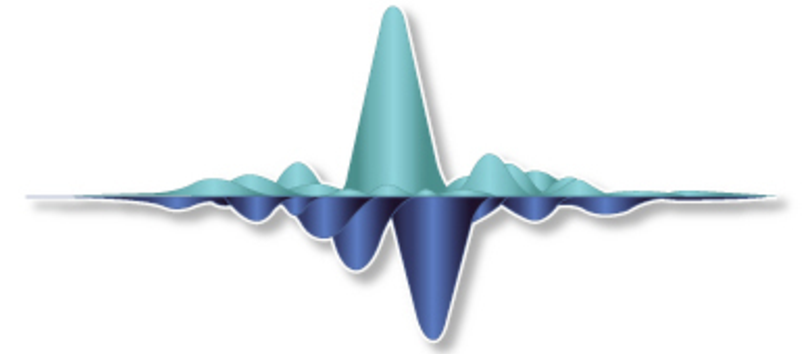
\includegraphics[width=1.6cm]{logo}}}}  

\begin{frame} \frametitle{Outline}
    \begin{itemize}
        \item Motivation
        \item Algorithm
        \item Synthetic Examples
        \item Real Examples
    \end{itemize}
\end{frame}

\begin{frame} \frametitle{Motivation}
    \begin{itemize}
        \item Processing tools that rely on sparsity or simplisity promotion can fail in the presence of static shifts.
	\item Many methods can solve for static shifts, but can we still process data with static shifts? 
	\item Here we adapt radon basis functions and reconstruction to work in the presence of small static shifts.
    \end{itemize}
\end{frame}


%\begin{frame} \frametitle{Motivation}
%    \begin{itemize}
%        \item Here's a bullet.
%        \item And another bullet.
%        \item and one more.
%    \end{itemize}
%    \pause
%    \begin{itemize}
%        \item Another set of bullets.
%            \pause
%        \item But these are hidden from one another.
%            \pause
%        \item Which can be used to make animations.
%    \end{itemize}
%\end{frame}

%\begin{frame} \frametitle{POCS}
%    \Huge{$\nabla^2 u - \alpha \frac{\partial u}{\partial t} = %\delta(\mathbf{x},t)$}
%\end{frame}

\begin{frame} \frametitle{General cost function}
    \Large{$J = |Ax-b|^2_2 + \mu|x|_1 $}

\bigskip

\bigskip
$A$ is a linear operator and depends on your application.
$x$ is the model.
\bigskip

\bigskip
{\color{red}Problem: when statics are present A does not produce a sparse model, x.}

\end{frame}

\begin{frame} \frametitle{General cost function}
    \Large{$J = |{\color{red}{\cal{S}}}Ax-b|^2_2 + \mu|x|_1 $}

\bigskip

\bigskip
$A$ is a linear operator and depends on your application.
${\color{red}{\cal{S}}}$ is a shifting operator.
$x$ is the model.
\bigskip

\bigskip
{\color{red}Solution: we add a shifting operator to add static shifts to the predicted data $Ax$.} 

\end{frame}


\begin{frame} \frametitle{Solving the original cost function: FISTA}
    \Large{$J = |Ax-b|^2_2 + \mu|x|_1 $}

\bigskip

$g_k=|Ax_k-b|^2_2$

\bigskip
\tiny
\par
\vbox{\begin{tabbing}
indent \= atechars \= atechars \=  atechars \= \kill
\>INPUT:$\mu,\alpha,b$	\\
\>$y_o=x_o=0$	\\
\>$t=1$	\\
\>$T=\mu/2\alpha$	\\
\>for ($k=0:N_{iter}$)	\\
\>	\>$x_{k+1} =$ Soft($y_k - \nabla g_k/\alpha$,$T$) 	\\
\>	\>$t_{k+1} = (1+\sqrt{1+4t_k^2})/2$ 	\\
\>	\>$y_{k+1}=x_{k+1}+[(t_{k+1}-1)/t_k](x_{k+1}-x_k)$	\\
\>end	\\
\end{tabbing} }
\par

\end{frame}

\begin{frame} \frametitle{Solving the modified cost function: FISTA}
    \Large{$J = |{\color{red}{\cal{S}}}Ax-b|^2_2 + \mu|x|_1 $}

\bigskip

${\color{red}g^{{\cal{S}}}_k=|{\cal{S}}_kAx_k-b|^2_2}$

\bigskip
\tiny
\par
\vbox{\begin{tabbing}
indent \= atechars \= atechars \=  atechars \= \kill
\>INPUT:$\mu,\alpha,b$	\\
\>$y_o=x_o=0$	\\
\>$t=1$	\\
\>$T=\mu/2\alpha$	\\
\>${\color{red}{\cal{S}}_o=I}$ \\
\>for ($k=0:N_{iter}$)	\\
\>	\>$x_{k+1} =$ Soft($y_k -  {\color{red}\nabla g^{{\cal{S}}}_k}  /\alpha$,$T$) 	\\
\>	\>$t_{k+1} = (1+\sqrt{1+4t_k^2})/2$ 	\\
\>	\>$y_{k+1}=x_{k+1}+[(t_{k+1}-1)/t_k](x_{k+1}-x_k)$	\\
\>	\>${\color{red}{\cal{S}}_{k+1}\leftarrow Ax_{k+1} \odot b}$	\\
\>end	\\
\end{tabbing} }
\par

\end{frame}


\begin{frame} \frametitle{Application to Radon}
    \Large{Cost$_1 = |Ax-b|^2_2 + \mu|x|_1 $}

\bigskip
    \Large{Cost$_2 = |{\color{red}{\cal{S}}}Ax-b|^2_2 + \mu|x|_1 $}

\bigskip

Here $A$ is adjoint of the parabolic radon transform, and ${\cal{S}}$ is a shifting operator, $b$ is a NMO corrected gather, and $x$ is the radon panel.

\end{frame}



%\begin{frame} \frametitle{Projection Onto Convex Sets}
%    \Large{$D^{k} = \alpha_1 D^{obs} + (1-\alpha_1 S)F_{D}^{-1}TF_{D}D^{k-1}$}
%
%\bigskip
%
%\bigskip
%$\alpha_1 \rightarrow$ 1  when data are free of noise.
%\end{frame}
%
%\begin{frame} \frametitle{Projection Onto Convex Sets\\ {\color{red}with statics computation}}
%    \Large{$D^{k} = \alpha_1 D^{obs}{\color{red}e^{-i\omega(1-\alpha_2)\tau^k}} + (1-%\alpha_1 S)F_{D}^{-1}TF_{D}D^{k-1}$}
%
%\bigskip
%
%\bigskip
%$\alpha_1 \rightarrow$ 1  when data are free of noise.
%{\color{red}
%
%$\alpha_2 \rightarrow$ 1  when data are free of statics.}
%\end{frame}
%

\inputdir{syn5d}
% we could also use includegraphics here instead
%\begin{frame} \frametitle{Plots}
%    \plot{data1}{width=0.5\textwidth}{}
%\end{frame}

%\begin{frame} \frametitle{Original data}
%    \multiplot{2}{dtrue,dtrue_fk}{width=0.45\textwidth}{}
%\end{frame}

%\begin{frame} \frametitle{Noise}
%    \multiplot{2}{dnoise,dnoise_fk}{width=0.45\textwidth}{}
%\end{frame}

%\begin{frame} \frametitle{Decimation}
%    \multiplot{2}{ddec,ddec_fk}{width=0.45\textwidth}{}
%\end{frame}

%\begin{frame} \frametitle{Statics}
%    \multiplot{2}{dstat,dstat_fk}{width=0.45\textwidth}{}
%\end{frame}

%\begin{frame} \frametitle{Multiplots}
%    \multiplot{2}{data1,data1}{width=0.45\textwidth}{}
%\end{frame}
%
%\begin{frame} \frametitle{example 2d all}
%    \plot{example_2d_all}{width=0.45\textwidth}{}
%\end{frame}
%
%\begin{frame} \frametitle{est data with without statics}
%    \multiplot{2}{estimated_data_without_statics,estimated_data_with_statics}{width=0.45\textwidth}{}
%\end{frame}


\begin{frame} \frametitle{Original data\\ }
\begin{figure}[t]
\centering
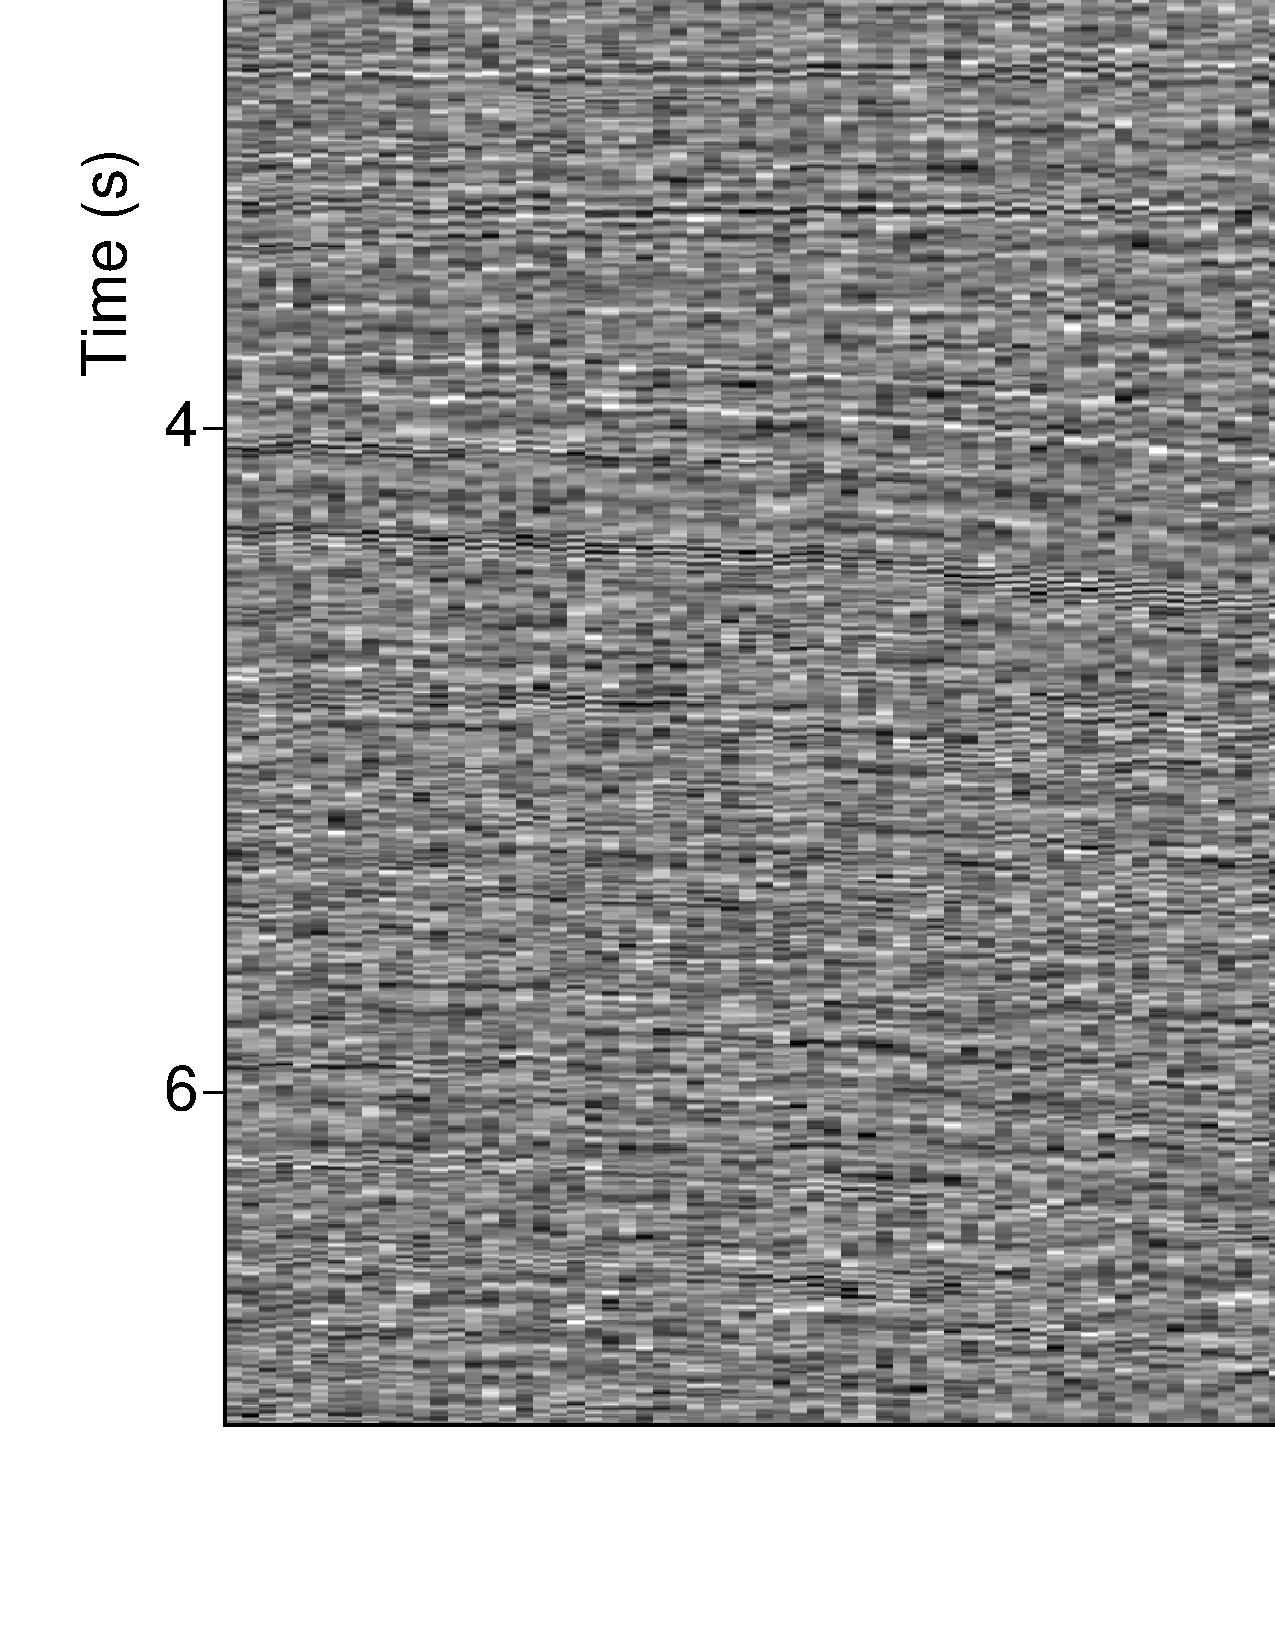
\includegraphics[width=0.75\textwidth,height=0.5\textwidth,keepaspectratio=false]{syn5d/Fig/original_data.pdf}
\end{figure}
\end{frame}

\begin{frame} \frametitle{Radon panel using cost function 1}
\begin{figure}[t]
\centering
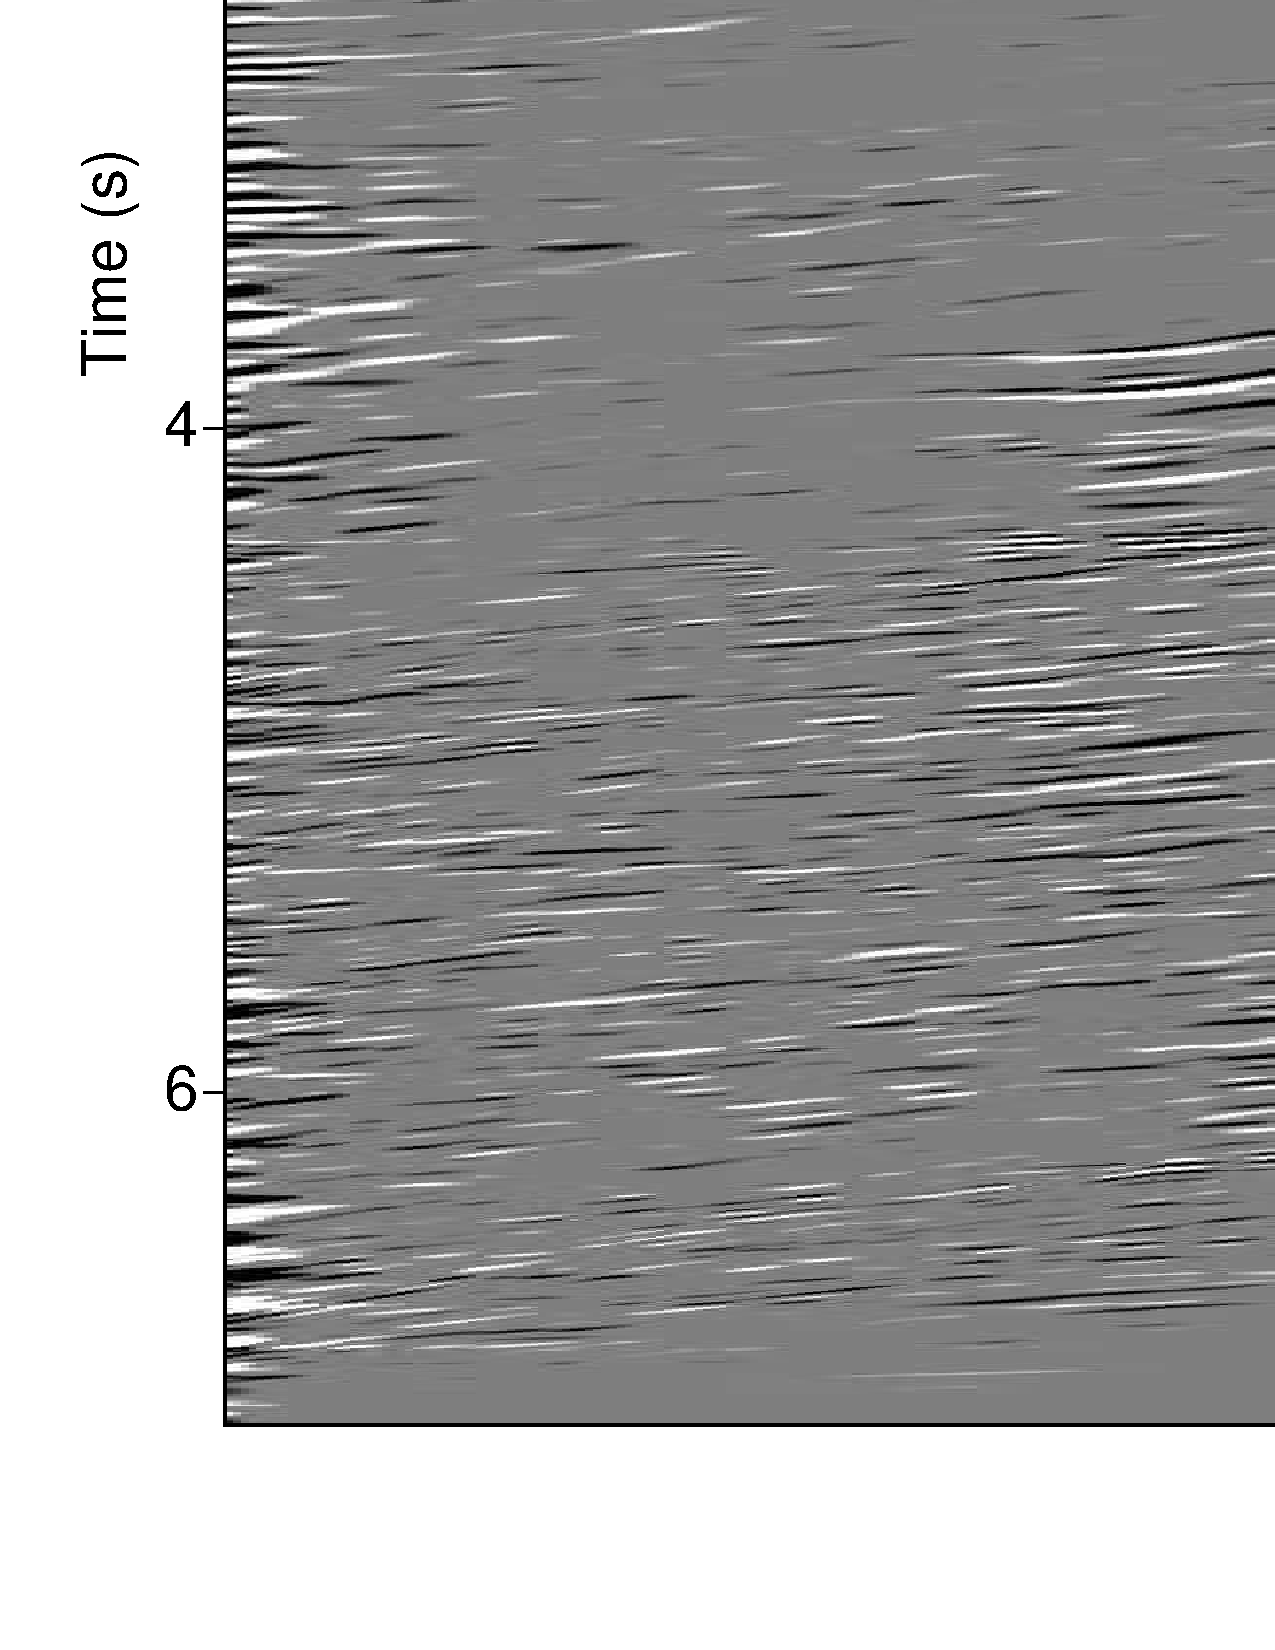
\includegraphics[width=0.75\textwidth,height=0.5\textwidth,keepaspectratio=false]{syn5d/Fig/high_resolution_radon_without_statics.pdf}
\end{figure}
\end{frame}

\begin{frame} \frametitle{Radon panel using cost function 2}
\begin{figure}[t]
\centering
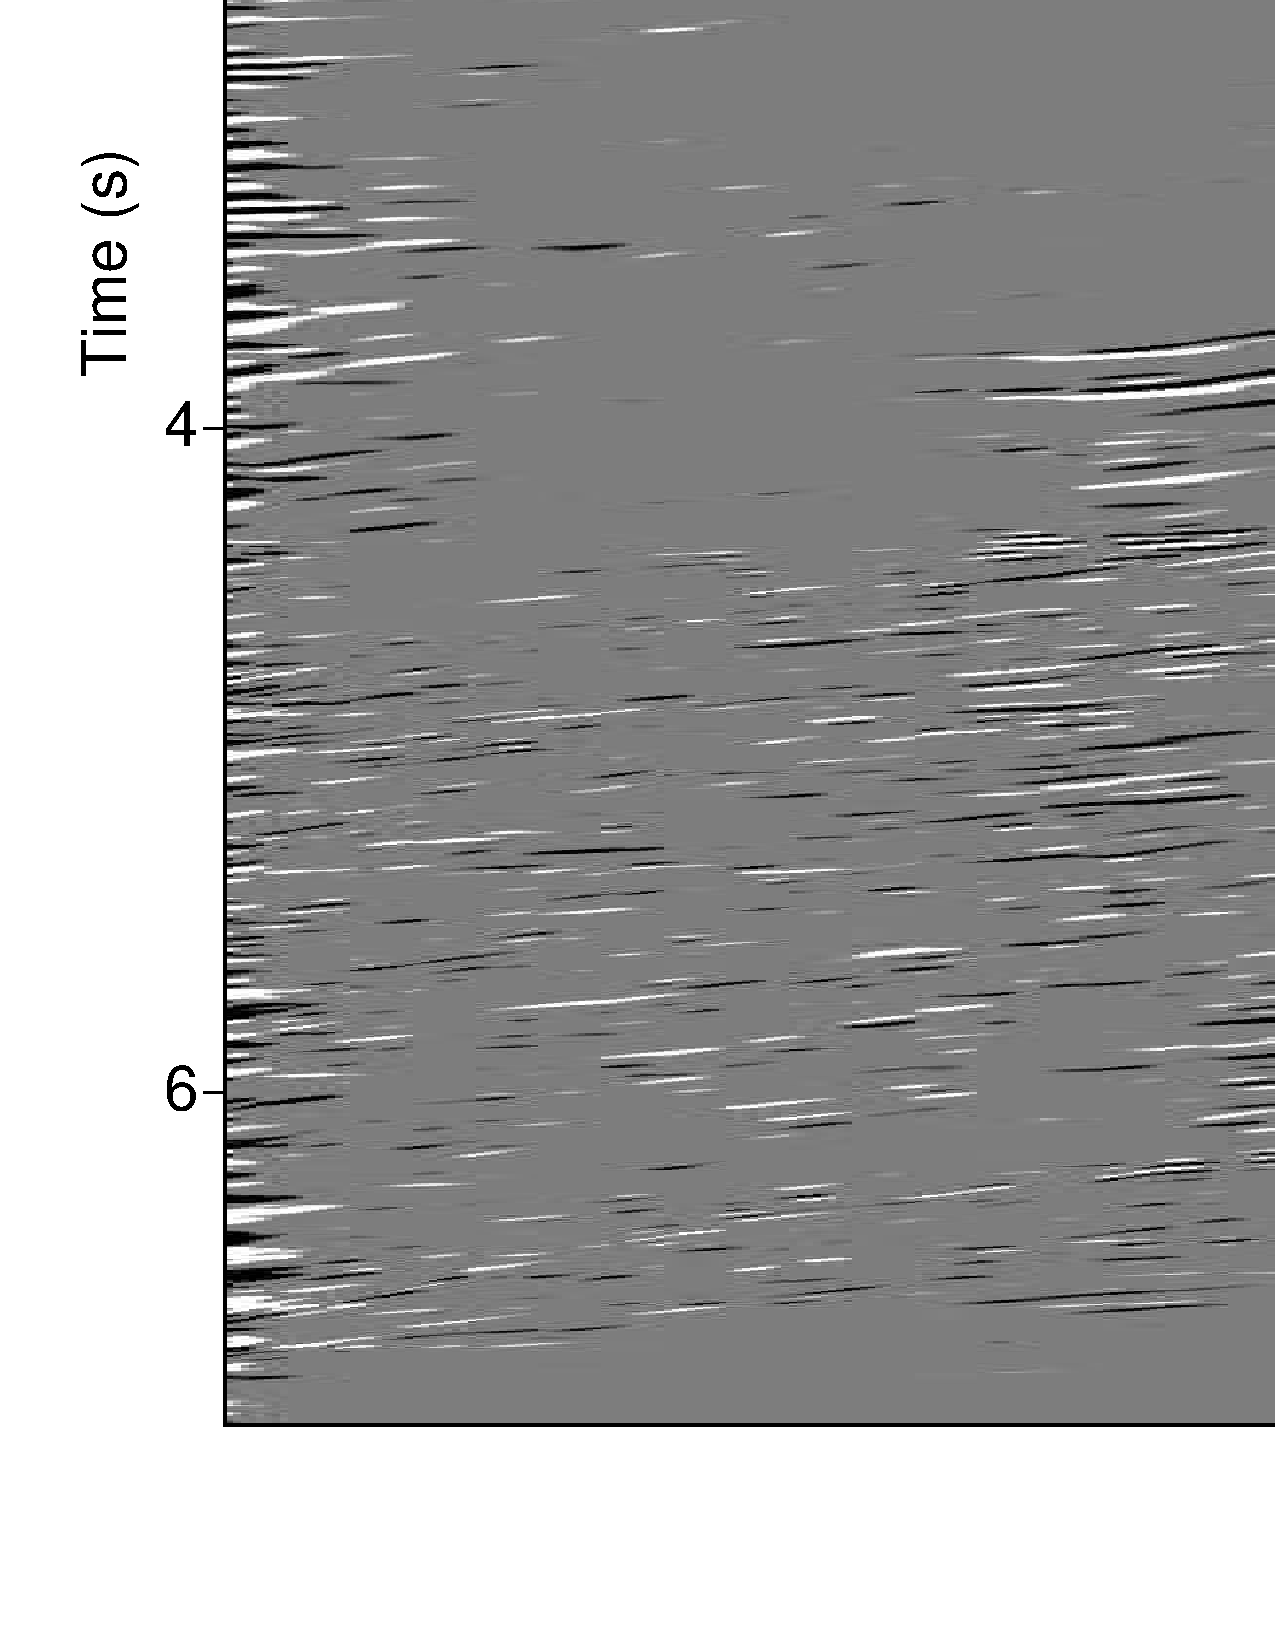
\includegraphics[width=0.75\textwidth,height=0.5\textwidth,keepaspectratio=false]{syn5d/Fig/high_resolution_radon_with_statics.pdf}
\end{figure}
\end{frame}

\begin{frame} \frametitle{Estimated data using cost function 1}
\begin{figure}[t]
\centering
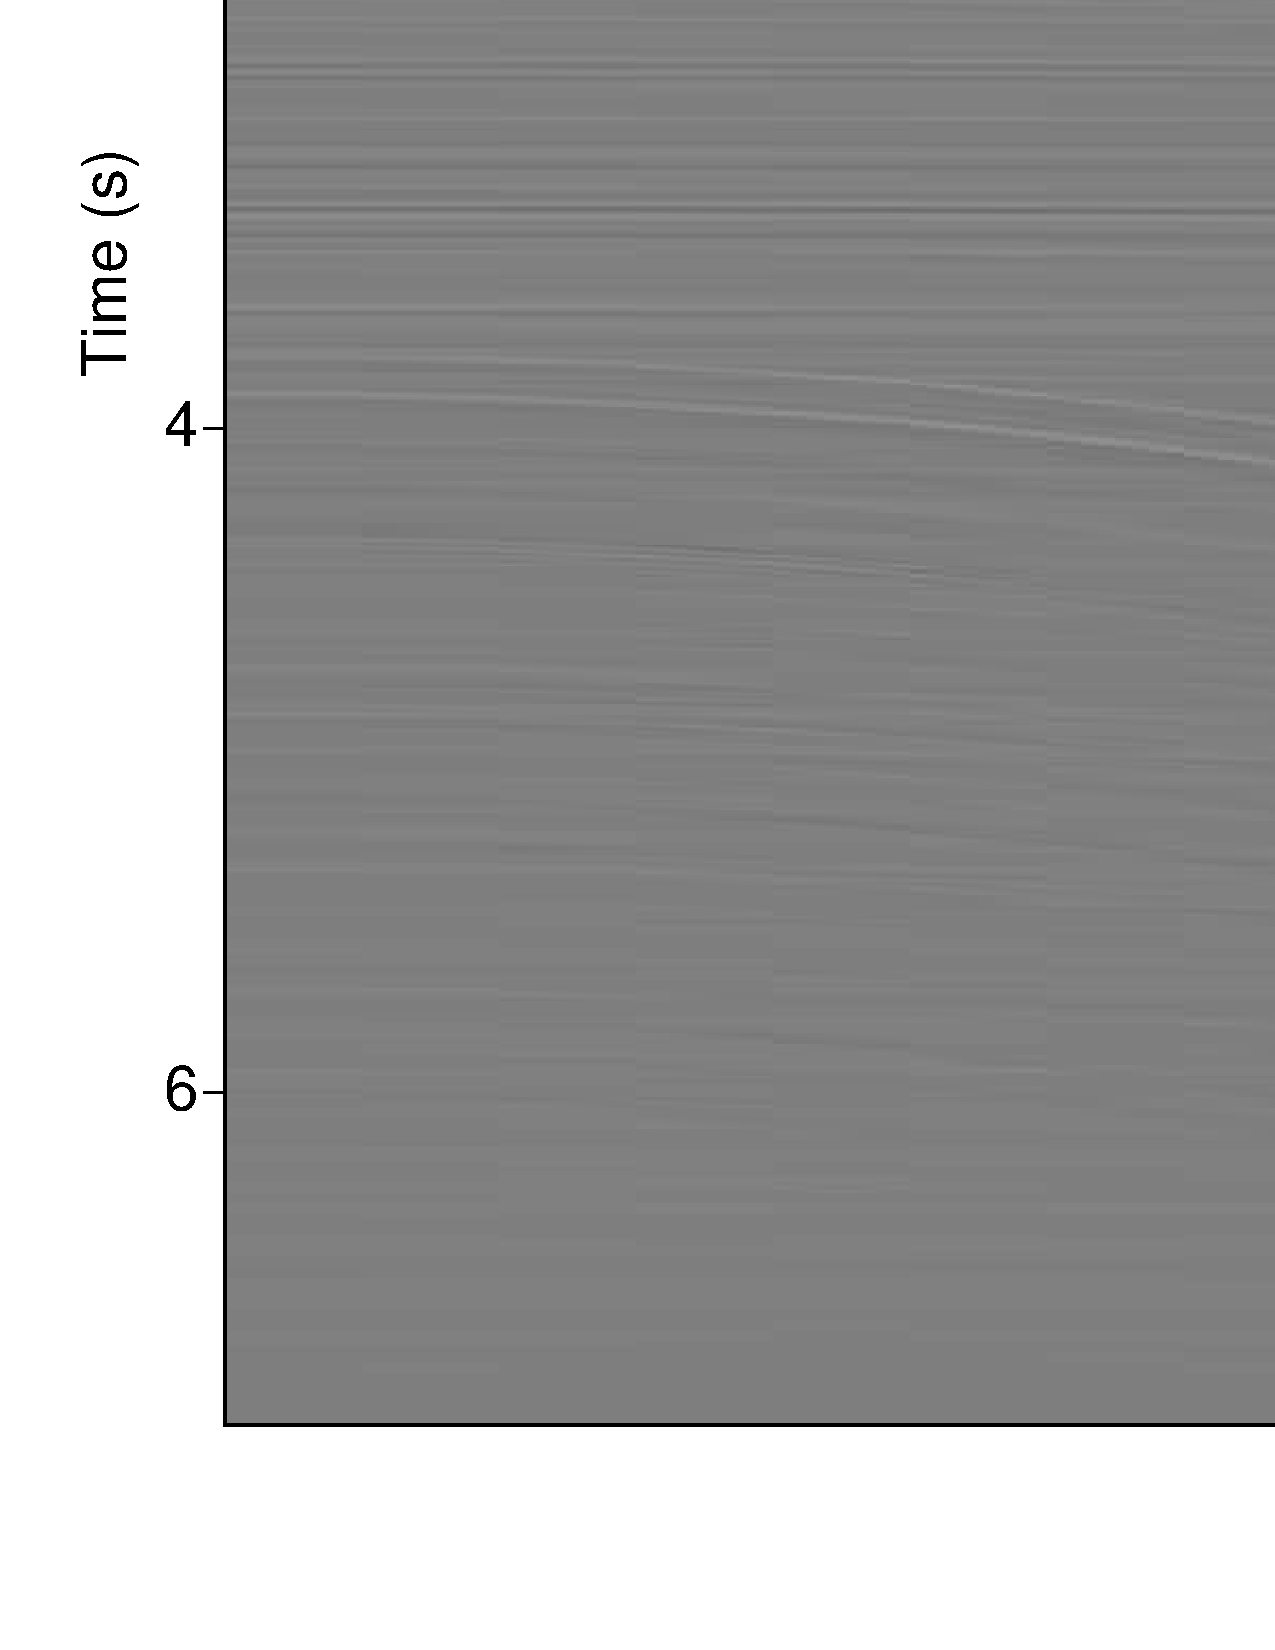
\includegraphics[width=0.75\textwidth,height=0.5\textwidth,keepaspectratio=false]{syn5d/Fig/estimated_data_without_statics.pdf}
\end{figure}
\end{frame}

\begin{frame} \frametitle{Estimated data using cost function 2}
\begin{figure}[t]
\centering
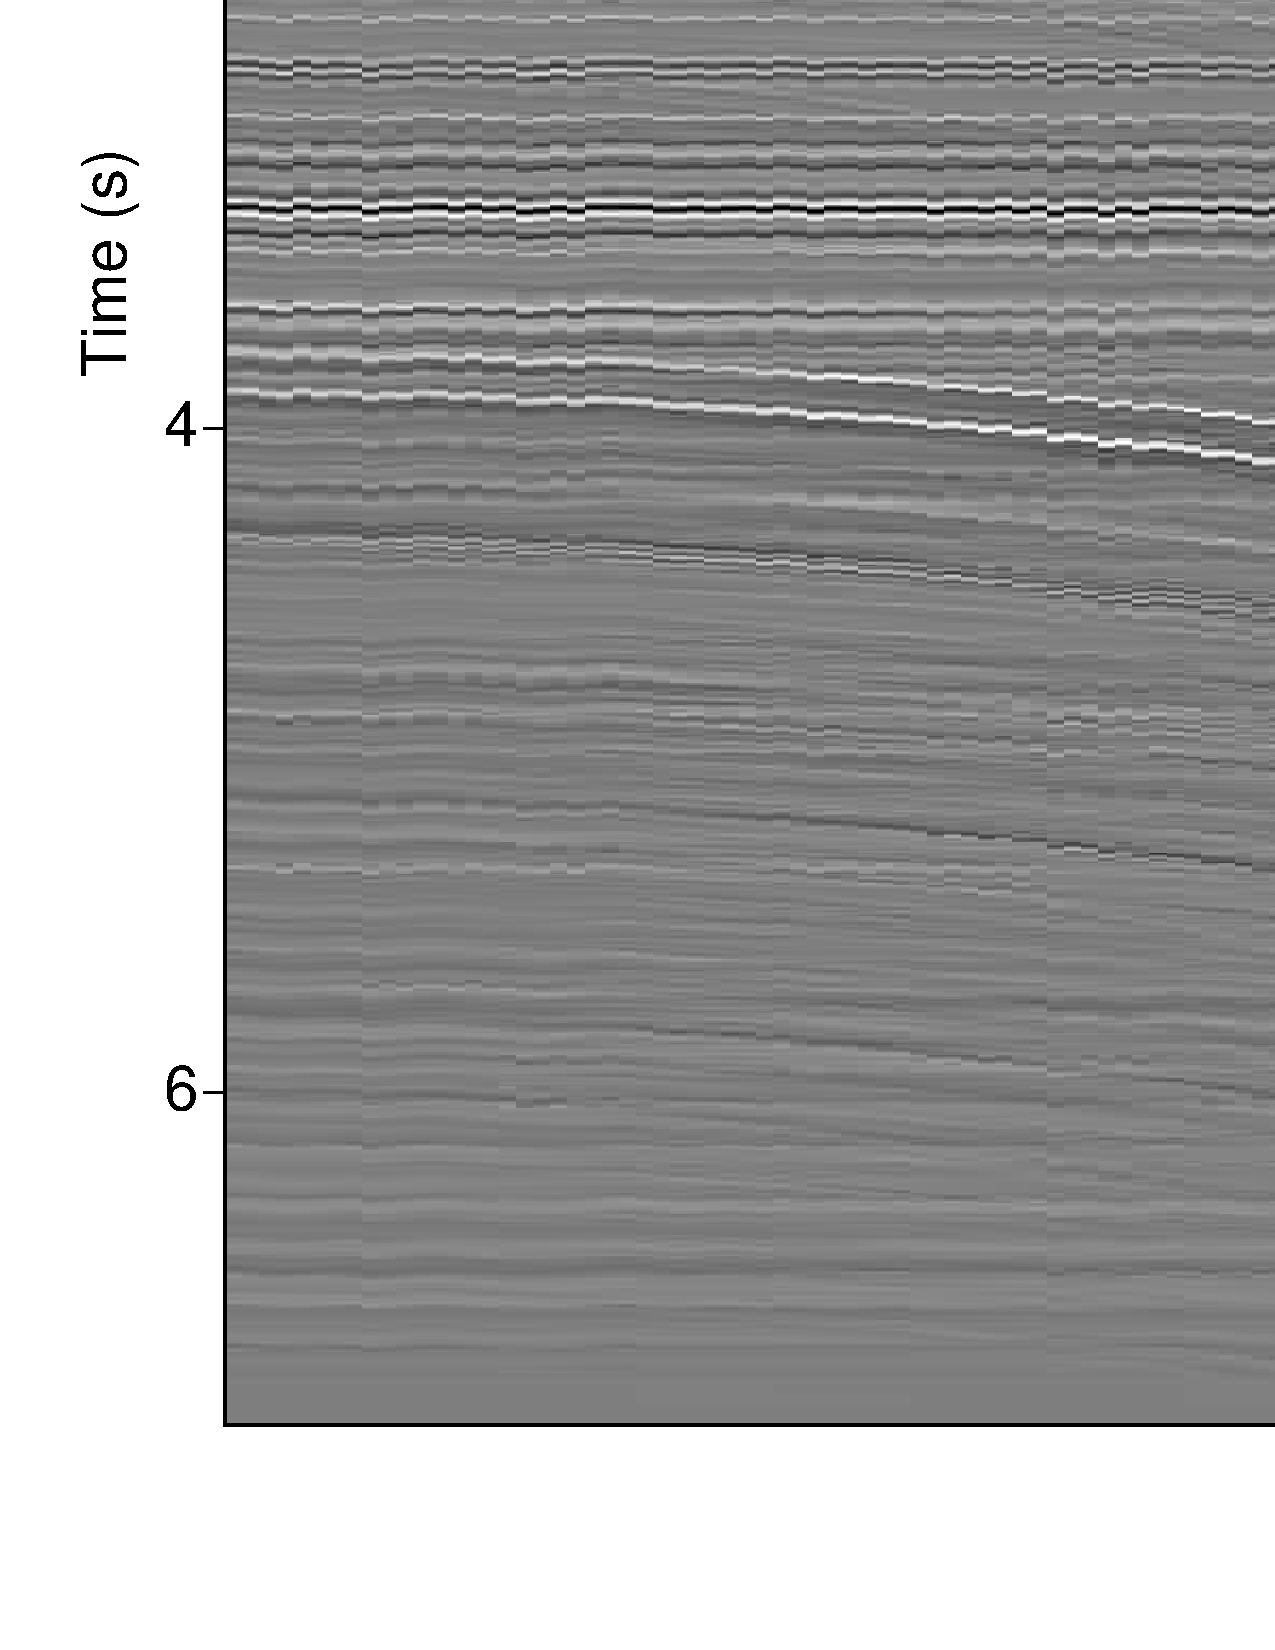
\includegraphics[width=0.75\textwidth,height=0.5\textwidth,keepaspectratio=false]{syn5d/Fig/estimated_data_with_statics.pdf}
\end{figure}
\end{frame}

\begin{frame} \frametitle{Application to reconstruction}
    \Large{Cost$_1 = |Ax-b|^2_2 + \mu|x|_1 $}

\bigskip
    \Large{Cost$_2 = |{\color{red}{\cal{S}}}Ax-b|^2_2 + \mu|x|_1 $}

\bigskip

Where $A=TF^H$. 

Here $F^H$ is the inverse Fourier transform and $T$ is the sampling operator. ${\cal{S}}$ is a shifting operator, $b$ is the input data, and $x$ are the Fourier coefficients.

\end{frame}


\begin{frame} \frametitle{Input data\\}
\begin{figure}[t]
\centering
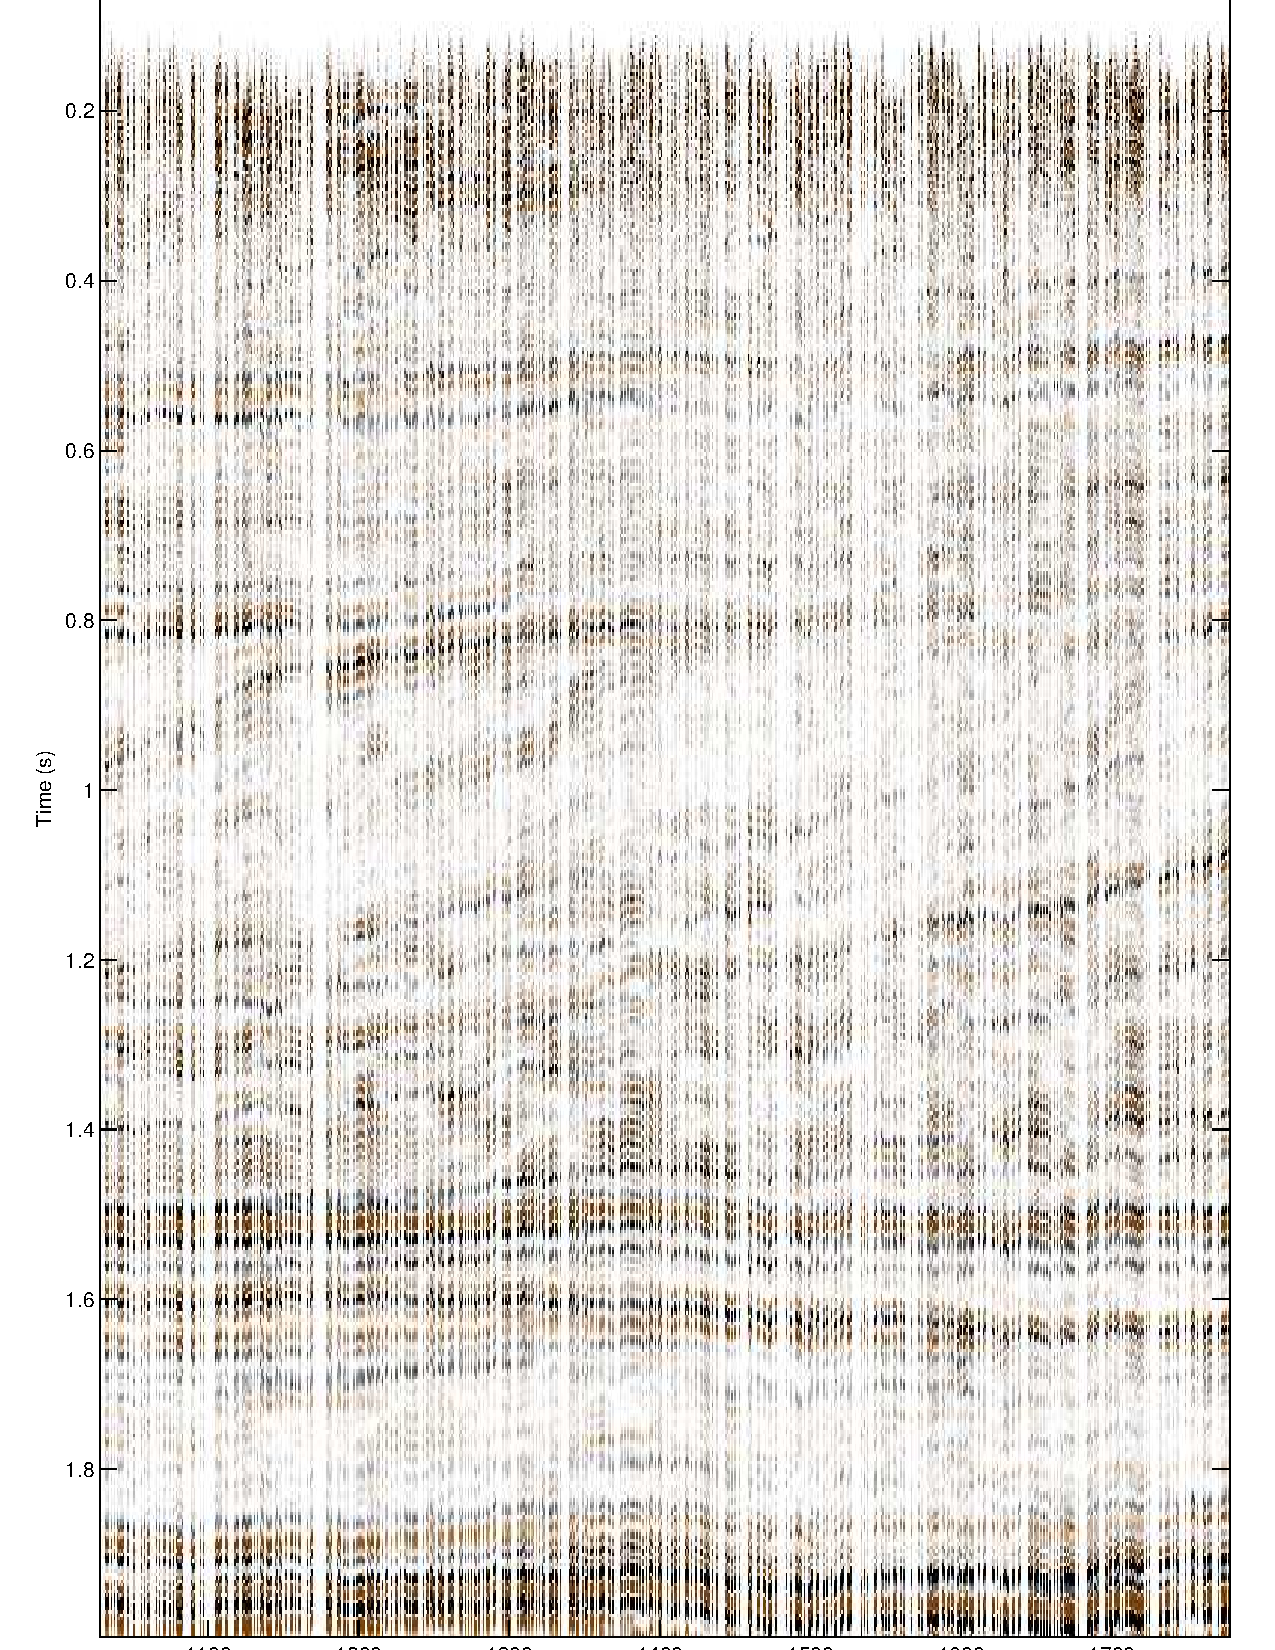
\includegraphics[width=1\textwidth,height=0.5\textwidth,keepaspectratio=false]{syn5d/Fig/image_d_stat.pdf}
\end{figure}
\end{frame}

\begin{frame} \frametitle{Data after applying reconstruction\\}
\begin{figure}[t]
\centering
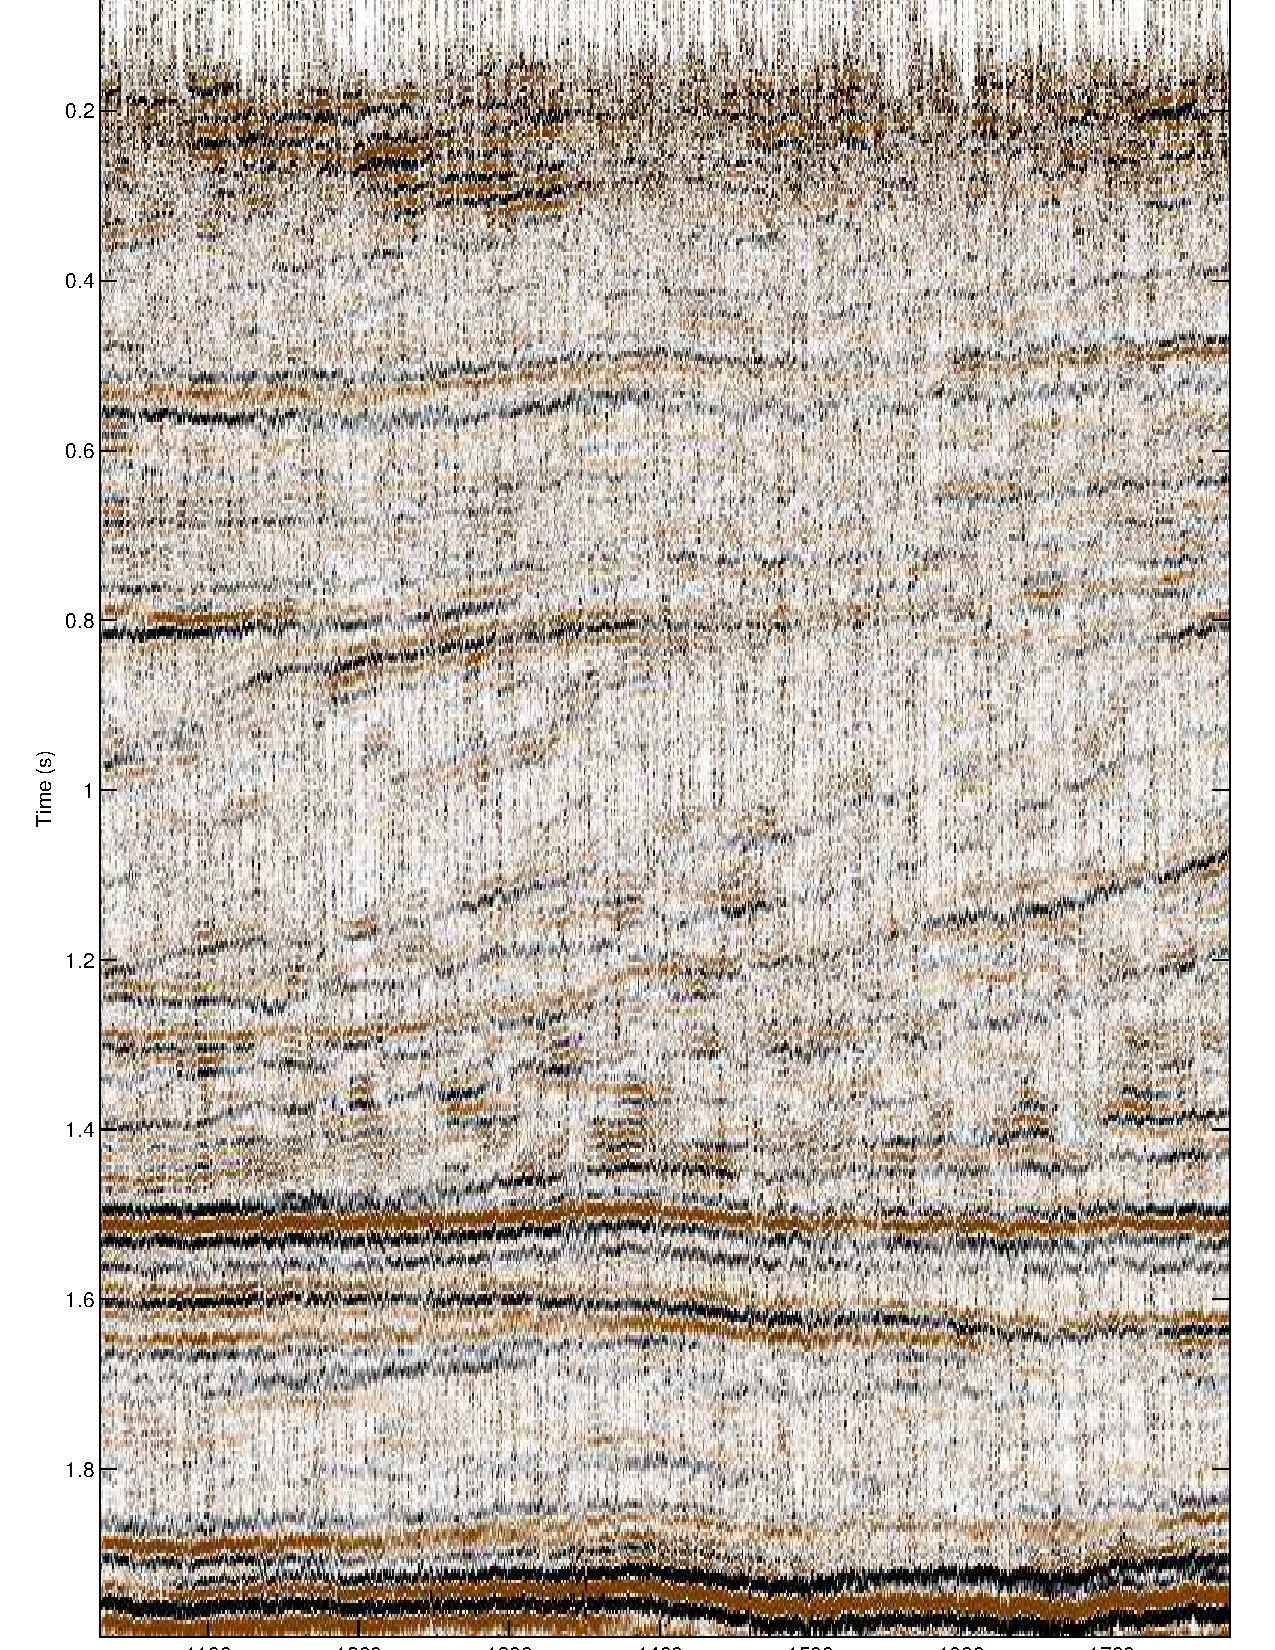
\includegraphics[width=1\textwidth,height=0.5\textwidth,keepaspectratio=false]{syn5d/Fig/image_d_stat_p.pdf}
\end{figure}
\end{frame}

\begin{frame} \frametitle{Data after applying modified reconstruction}
\begin{figure}[t]
\centering
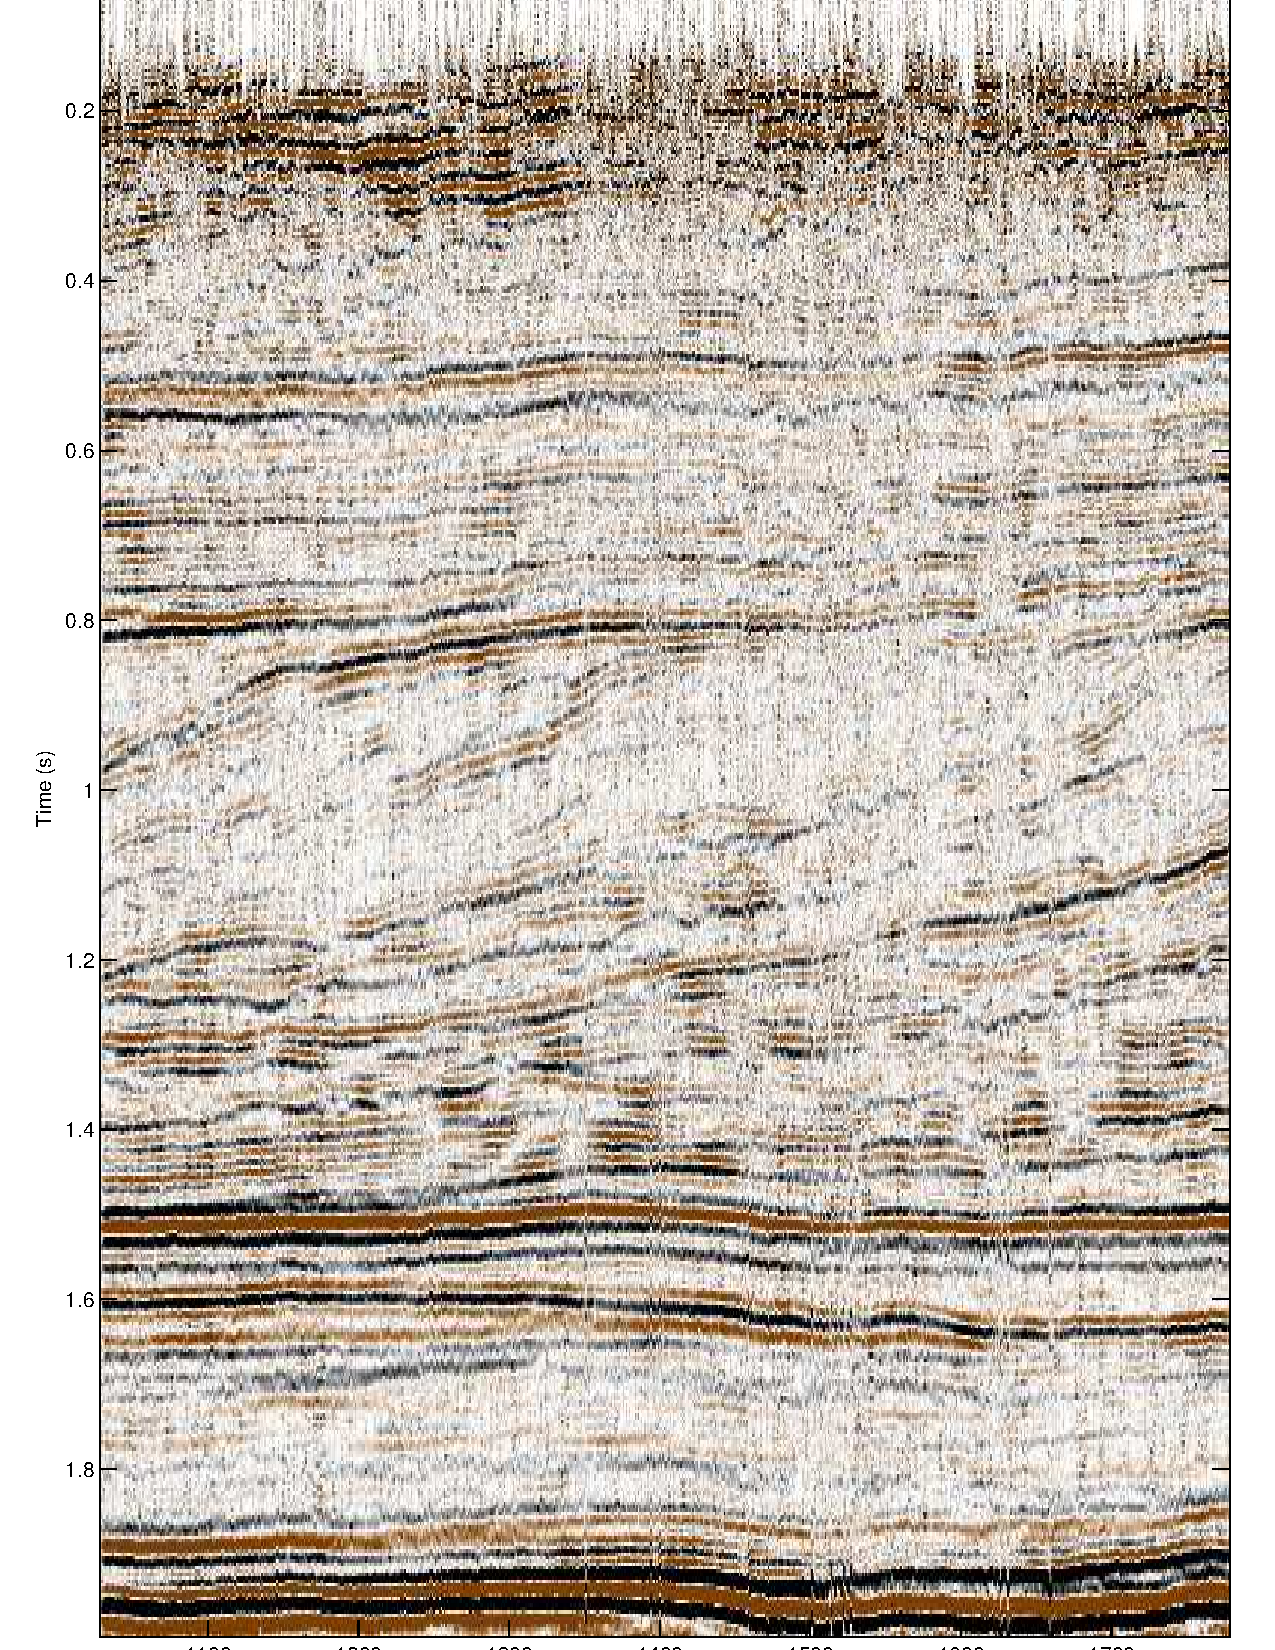
\includegraphics[width=1\textwidth,height=0.5\textwidth,keepaspectratio=false]{syn5d/Fig/image_d_stat_pws.pdf}
\end{figure}
\end{frame}


%\begin{frame} \frametitle{No missing traces}
%\begin{figure}[t]
%\centering
%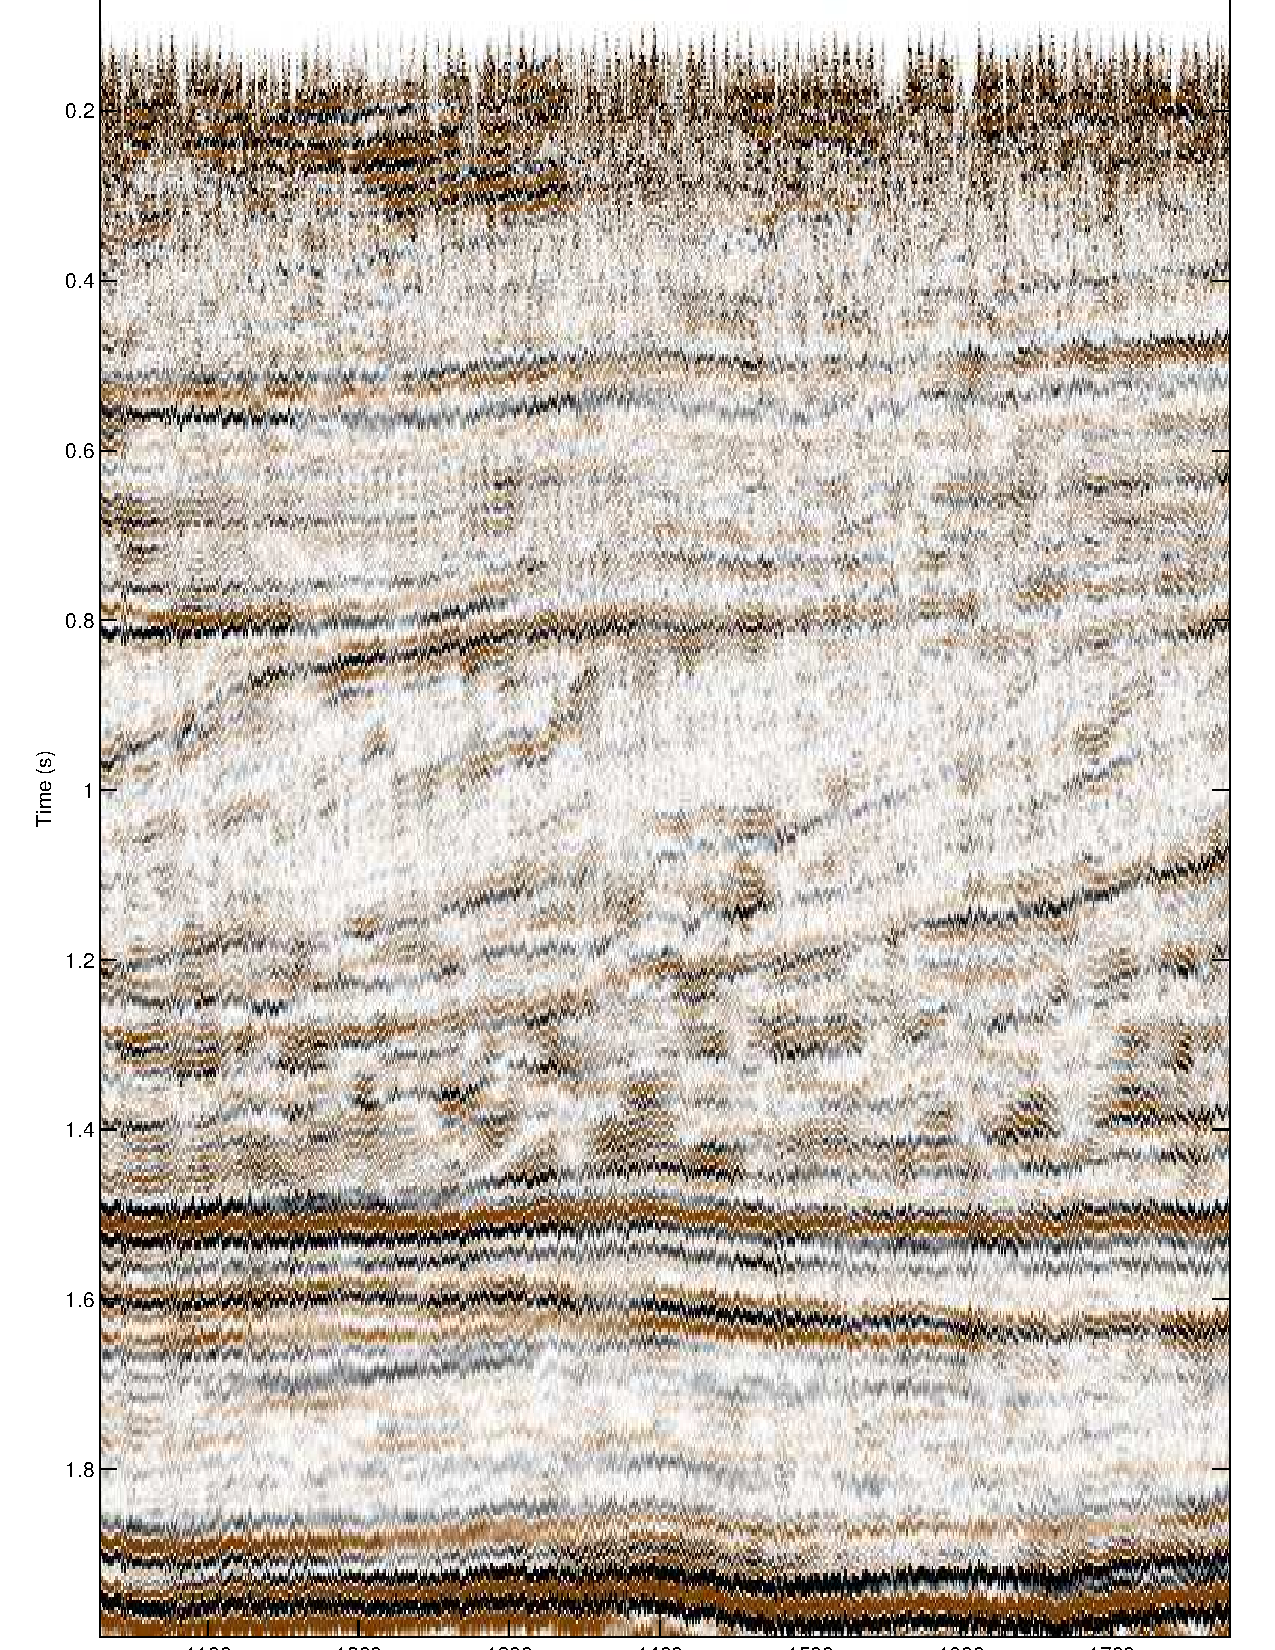
\includegraphics[width=1\textwidth,height=0.5\textwidth,keepaspectratio=false]{syn5d/Fig/no_missing.pdf}
%\end{figure}
%\end{frame}

%\begin{frame} \frametitle{No missing traces: corrected}
%\begin{figure}[t]
%\centering
%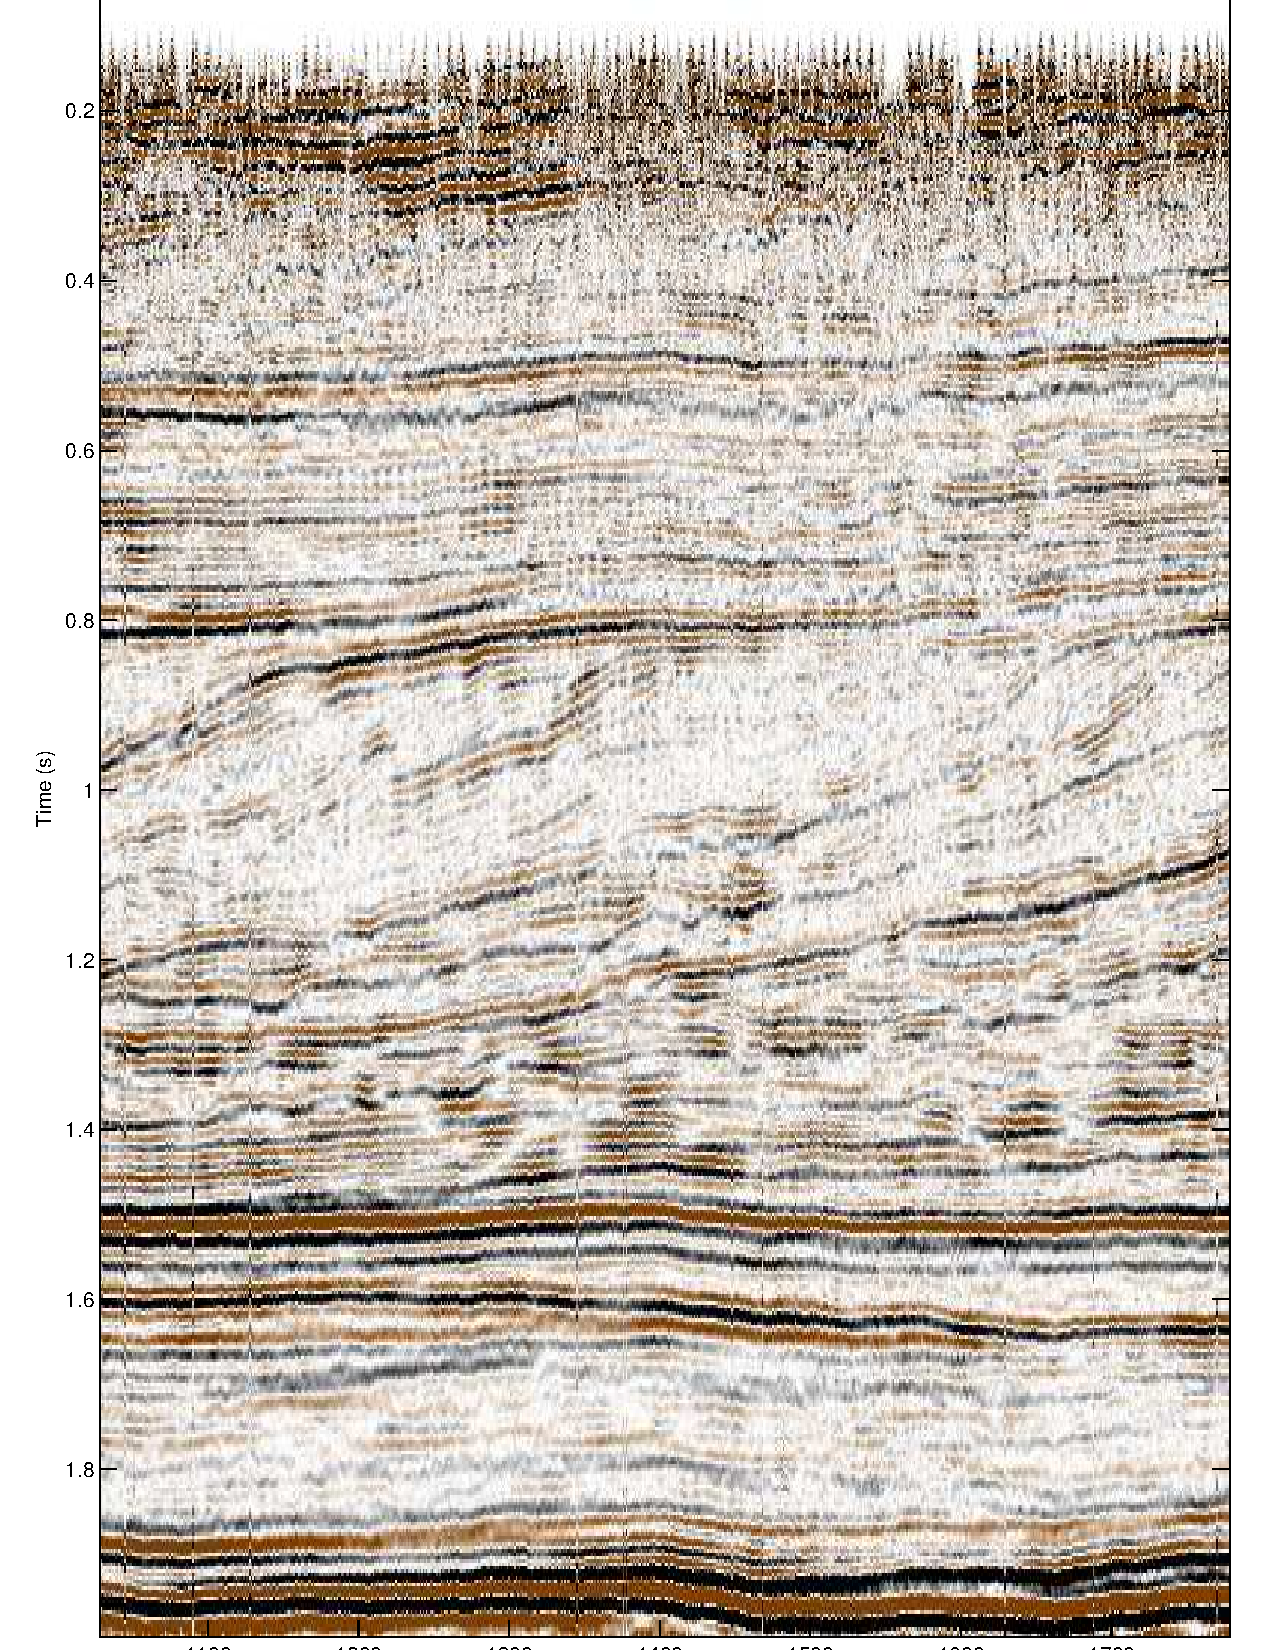
\includegraphics[width=1\textwidth,height=0.5\textwidth,keepaspectratio=false]{syn5d/Fig/no_missing_pws.pdf}
%\end{figure}
%\end{frame}

\begin{frame} \frametitle{Conclusions}
    \begin{itemize}
        \item We have presented a method to allow for sparsity promotion in the presence of small static shifts.
	\item We applied this method to Radon basis functions and Fourier Reconstruction.
	\item For both Radon and Fourier transforms including statics in the basis functions resulted in improved signal preservation and reconstruction.
	\item Future work: surface consistency of the estimated statics and the study of different operators and applications of this method.
    \end{itemize}
\end{frame}

\begin{frame} \frametitle{Acknowledgements}
    \begin{itemize}
        \item The sponsors of the Signal Analysis and Imaging Group (SAIG) at the University of Alberta
	\item The United States Geological Survey (USGS) for example data
    \end{itemize}
\end{frame}


